%\usepackage{multicol}

\section{Mutlicolumns}
\begin{multicols}{2}
For low epsilon (illustrated in \cref{fig:toy_maze_low_epsilon} and \cref{fig:easy_maze_low_epsilon}):
    \begin{enumerate}
        \item A steeper slope downwards and/or a more convergent solution  downwards is observed towards the end (trials 7 to 10). %graph 1
        \item A steeper slope is found at the start of the learning trials (2 to 4), but the slope is levelled after the first 2 trials. %graph 1 Graph 4.
    \end{enumerate}

\columnbreak
For a higher epsilon (illustrated in \cref{fig:toy_maze_high_epsilon} and  \cref{fig:easy_maze_high_epsilon}):
    \begin{enumerate}
        \item A steeper learning rate is found in trials 4/5 to 6/7. %graph 8 and 7
        \item A less steep downwards slope is found towards the end of the trials (7-10). %graph7 8 and 7
        \item More variation in the number of steps during the final trials 7-10 is found. %sortof graph7weak 7 and 8 +Easy 9
        \item The generally, the absolute number of steps after 10 trials, is lower for a higher learning rate.
    \end{enumerate}
\end{multicols}



\section{Multiple figers next to eachother}
Enter the following text above main:
\begin{verbatim}
    % To get side by side pictures:{
\usepackage{caption}
\usepackage{subcaption}
\usepackage{graphicx}
\end{verbatim}

\begin{figure}[H]
\centering
\begin{subfigure}{.48\textwidth}
  \centering
  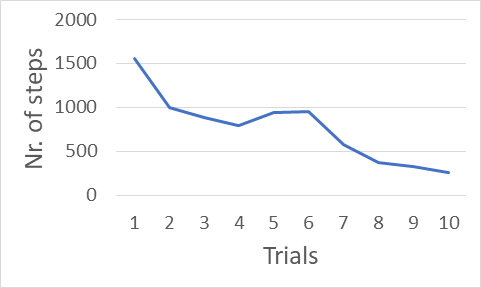
\includegraphics[width=0.99\linewidth]{images/2.2training/1Graph3.png}
    \caption{Toy maze with $\epsilon = 0.1$}
    \label{fig:toy_maze_low_epsilon}
\end{subfigure}
\begin{subfigure}{.48\textwidth}
  \centering
  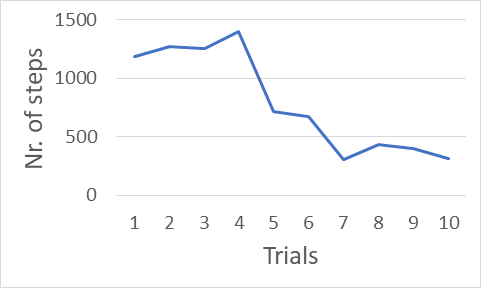
\includegraphics[width=1\linewidth]{images/2.2training/7Graph3.png}
      \caption{Toy maze with  $\epsilon = 0.7$}
    \label{fig:toy_maze_high_epsilon}
\end{subfigure}
%\label{fig:perceptron_learning_performance}
\begin{subfigure}{.48\textwidth}
  \centering
  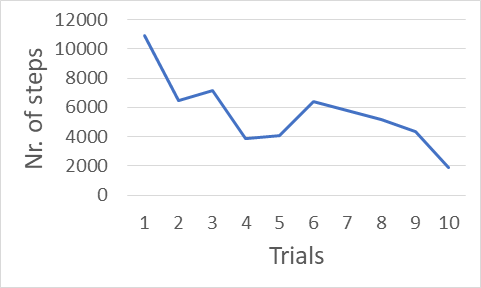
\includegraphics[width=0.99\linewidth]{images/2.2training/0Graph4.png}
    \caption{Easy maze with $\epsilon = 0.1$}
    \label{fig:easy_maze_low_epsilon}
\end{subfigure}
\begin{subfigure}{.48\textwidth}
  \centering
  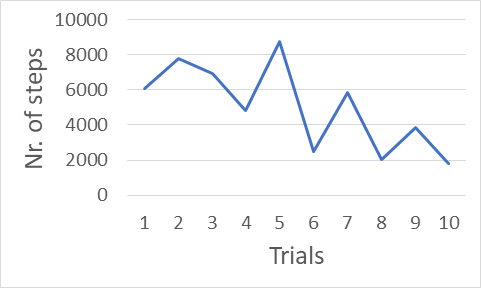
\includegraphics[width=1\linewidth]{images/2.2training/9Graph4.png}
      \caption{Easy maze with $\epsilon = 0.9$}
    \label{fig:easy_maze_high_epsilon}
\end{subfigure}
\caption{Number of steps required for robot to reach target with learning, as a function of $\epsilon$.}
%\label{fig:perceptron_learning_performance}
\end{figure}


\section{Evend out columns:}
\begin{multicols}{2}
\noindent Low $\epsilon$ advantage(s): 
    \begin{itemize}
        \item A quick decrease in initial required number of steps at the start of agent learning trials.
        \item A higher rate of conversion to the optimal solution, once it has been learned, due to a lower exploration rate
    \end{itemize}
\noindent Low $\epsilon$ disadvantage(s):
\begin{itemize}
    \item A plateau due to a lower initial exploration of options
    \item Higher risk of getting stuck in a "local minimum" due to reduced rate of exploration.
\end{itemize}
\columnbreak
High $\epsilon$ advantage(s): 
\cref{fig:easy_maze_high_epsilon}):
    \begin{itemize}
        \setcounter{enumi}{2}
        \item An increased chance of finding the actual optimum route in stead of a local minimum, due to the increased rate of exploration.
    \end{itemize}
\bigskip
\bigskip
\bigskip
\bigskip
\bigskip
\bigskip
\bigskip
\bigskip
\noindent High $\epsilon$ disadvantage(s): 
\begin{itemize}
    \item A slower rate of "learning/performance improvement" due to inital higher rate of exploration.
    \item Lower convergence to the final optimal solution once it has been learned, due to increased exploration.
\end{itemize}
\end{multicols}

\setcounter{section}{1} 
\setcounter{subsection}{1}
\section{Custom subsection and enumeration numbering}
\begin{enumerate}
    \setcounter{enumi}{4} 
    \item Start
    \item last enumeration
\end{enumerate}
\subsection{alphanumeric numbering}
Use package \verb+\usepackage{enumitem}\verb+
\begin{enumerate}[label=(\alph*)]
    \item Start
    \item last enumeration
\end{enumerate}

\subsection{Alhpanumeric subsections}
\renewcommand{\thepart}{\Alph{part}}
%\renewcommand{\thechapter}{\Roman {chapter}}
\renewcommand{\thesection}{\arabic{section}}
\renewcommand{\thesubsection}{\alph{subsection})}
\renewcommand{\thesubsubsection}{\alph{subsection}\alph{subsubsection})}